\documentclass{article}
\usepackage[utf8]{inputenc}
\usepackage{graphicx}
\usepackage{enumerate}
\usepackage{amsmath}

\graphicspath{ {../figs/} }

\setlength{\parindent}{4em}
\setlength{\parskip}{1em}
\renewcommand{\baselinestretch}{1.3}

\makeatletter
% we use \prefix@<level> only if it is defined
\renewcommand{\@seccntformat}[1]{%
  \ifcsname prefix@#1\endcsname
    \csname prefix@#1\endcsname
  \else
    \csname the#1\endcsname\quad
  \fi}
% define \prefix@section
\newcommand\prefix@section{Part \thesection: }
\makeatother

\title{Lab07: Groundwater Flow through a porous medium}
\author{Prithvi Thakur}
\date{Dec 10, 2018}

\begin{document}

\maketitle

% Problem 1
\section{Boundary conditions for the given model}
The appropriate boundary conditions are found using linear interpolation of the given values. We can use the function interp1d or write a simple equation for a line using the given points. The boundary values are:

Left = [967 973 979 985 990 995 1000 995 990 985 980] 

Right = [960 965 975 985 995 990 985 980 975 970 965] 

Top = [980 979.250 978.500 977.750 977 976.250 975.500 \\ 
      974.750 974 973.250 972.500 971.750 971 970.250 \\
      \tab \tab 969.500 968.750 968 967.250 966.500 965.750 965]     

Bottom &= [967 966.65 966.30 965.95 965.60 965.25 964.90 \\
          \tab \tab 964.55 964.20 963.85 963.50 963.15 962.80 962.45 \\ 
          \tab \tab 962.10 961.75 961.40 961.05 960.70 960.35 960] 

\newpage
% Problem 2 
\section{Variation in Fluid Potential}
To compute the variation in fluid potential, we solve the diffusion equation at steady state, when the rate of change of solution with respect to time is zero. The only source of potential flow would be the boundary conditions computed above.

We get, $\frac{\partial^2u_x}{\partial x^2} + \frac{\partial^2u_y}{\partial y^2}= 0$. The source for the steady state would be the boundary conditions. Therefore, we can assemble the second finite difference matrix in global form as a function of x and y, and we can assemble the right hand side as a global boundary condition, i.e., linear array of all the boundary conditions. 

\begin{figure}
    \centering
    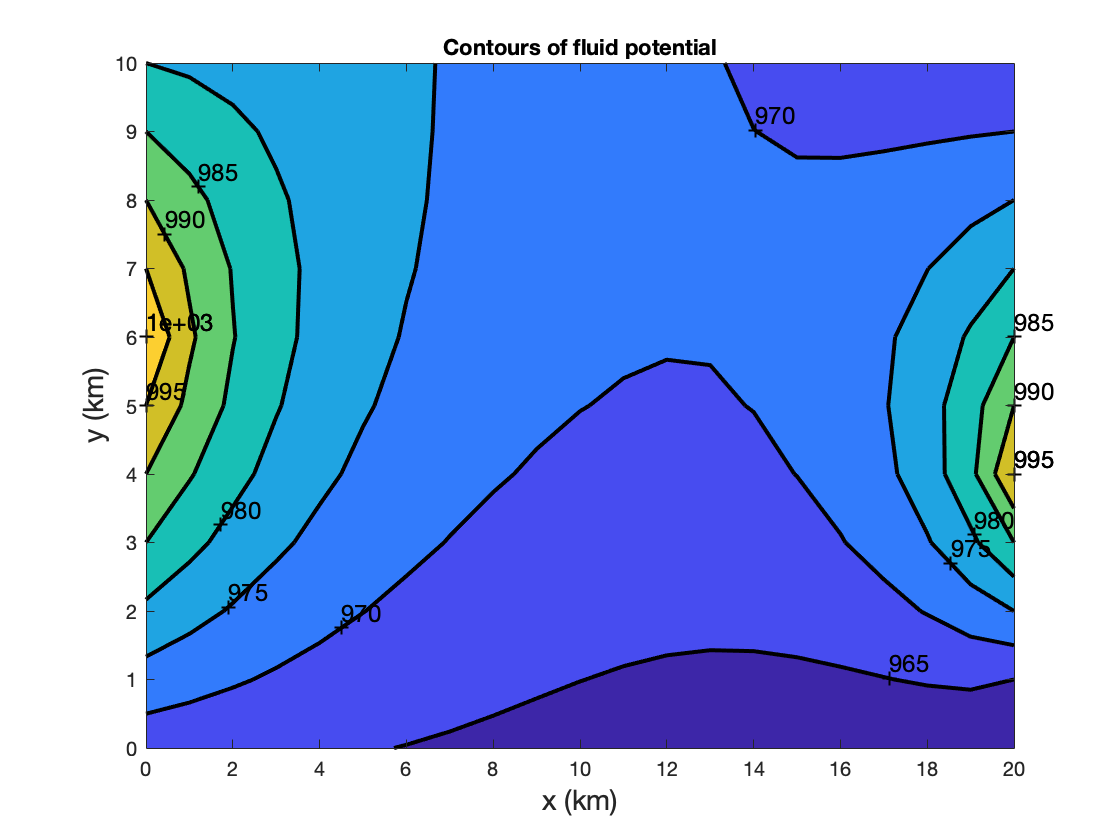
\includegraphics[scale=0.3]{1.png}
    \caption{Contours of fluid potential at steady state (in $m^2s^{-2}$)}
\end{figure}

% Problem 2
\section{Velocity vectors}

The velocity vectors would just be given by the components of the gradient of the fluid potential. We can plot it using quiver plot.
\begin{figure}
    \centering
    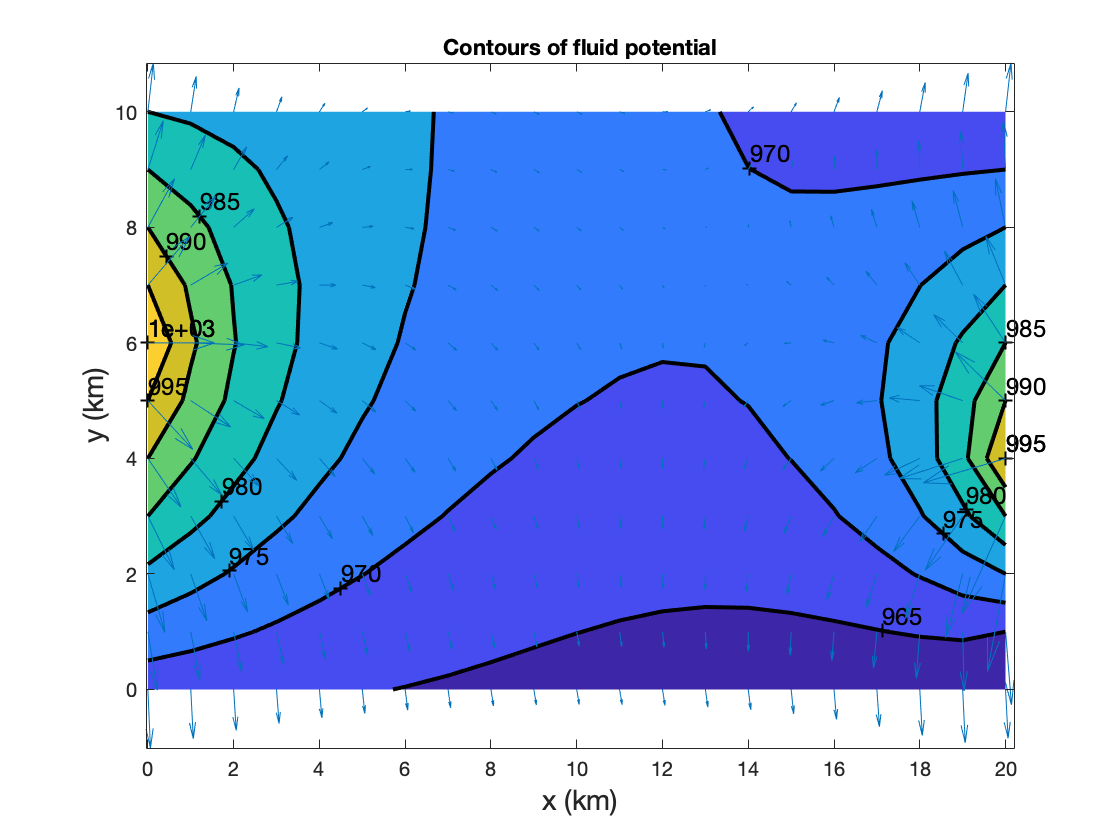
\includegraphics[scale=0.3]{3.png}
    \caption{Velocity vectots plotted in the fluid potential contour plots. It will be perpendicular to the contours.}
\end{figure}

\newpage
% Problem 3
\section{Tracer trajectory}

We begin with the initial location of tracer points and given the velocity vector at each grid point, we can propagate the tracer location. We use a timestep of one day. It takes 272 days to for the tracer to leave the domain.
\begin{figure}
    \centering
    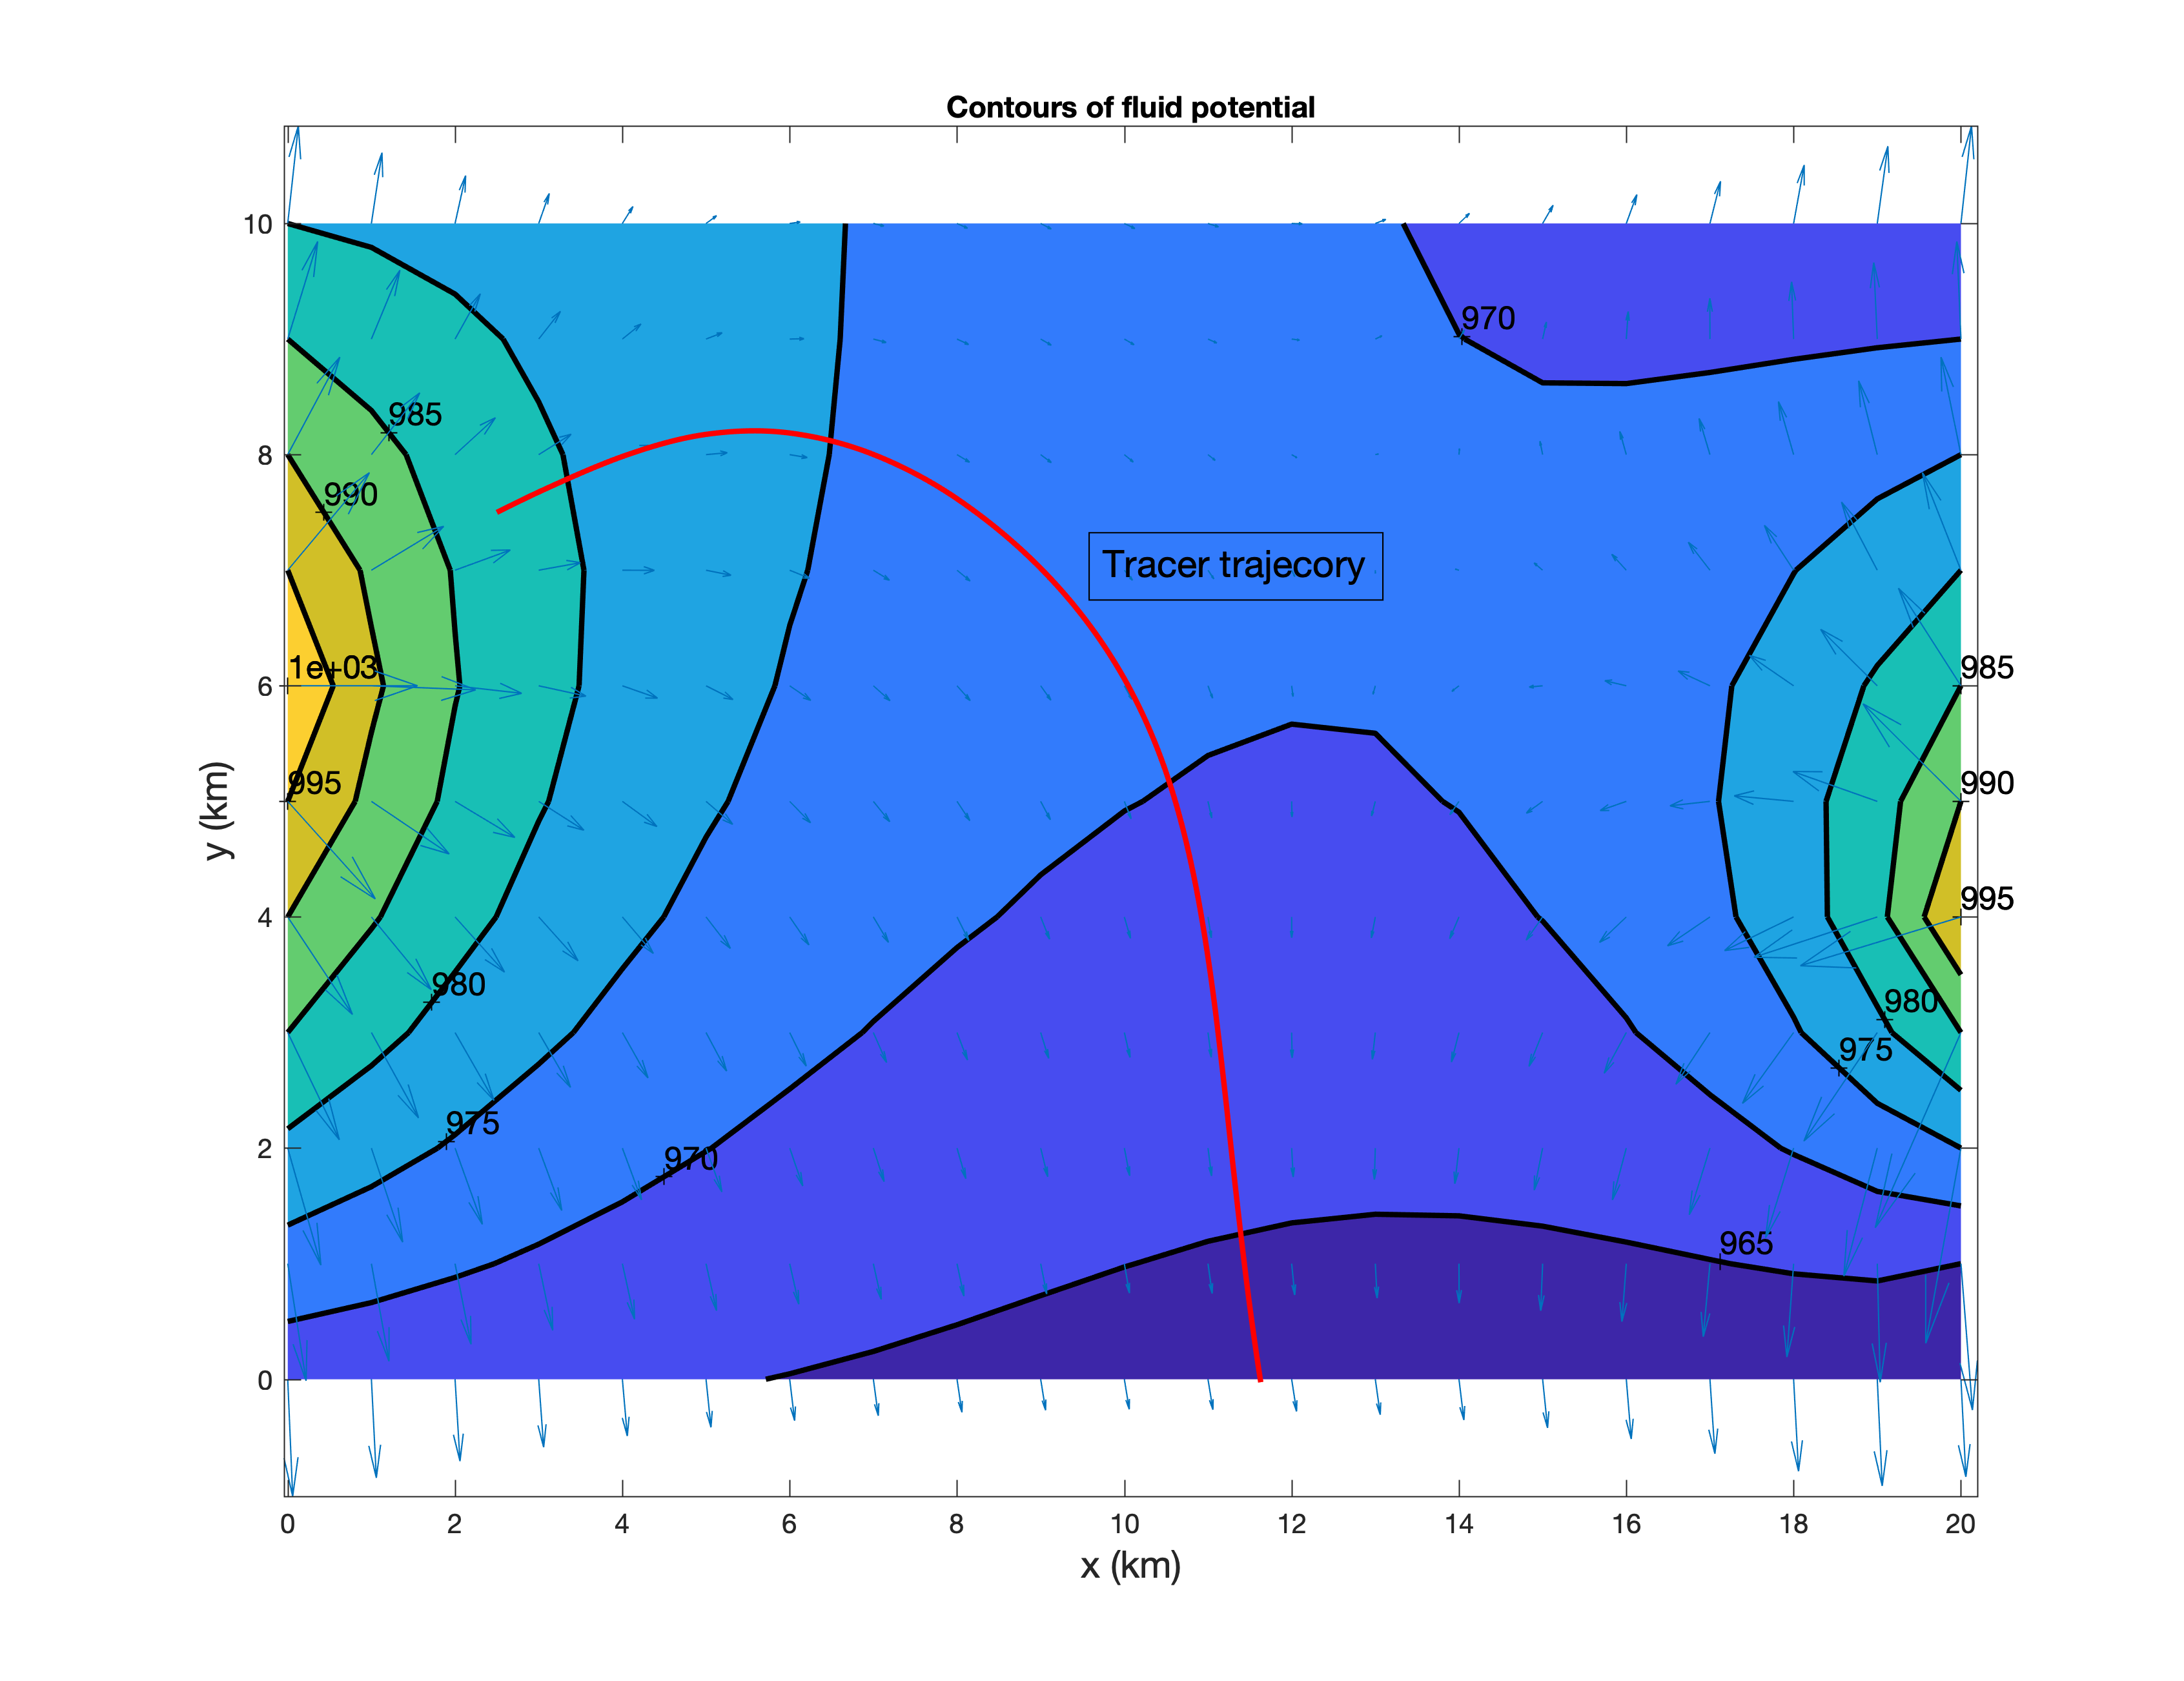
\includegraphics[scale=0.4]{2.png}
    \caption{Fluid potential contours with the velocity vectors. The tracer trajectory is given by the red line.}
\end{figure}

% Problem 5
\section{Time dependent diffusion equation}

In the steady state equation above, we will add the time rate change of potential and the source term to get the pollutant captured by extraction well. We can use a simple euler forward step to solve the time-dependent equation. We get the minimum extraction rate as $1.64\times10^{-7} m^2s^{-3}$. 

\begin{figure}
    \centering
    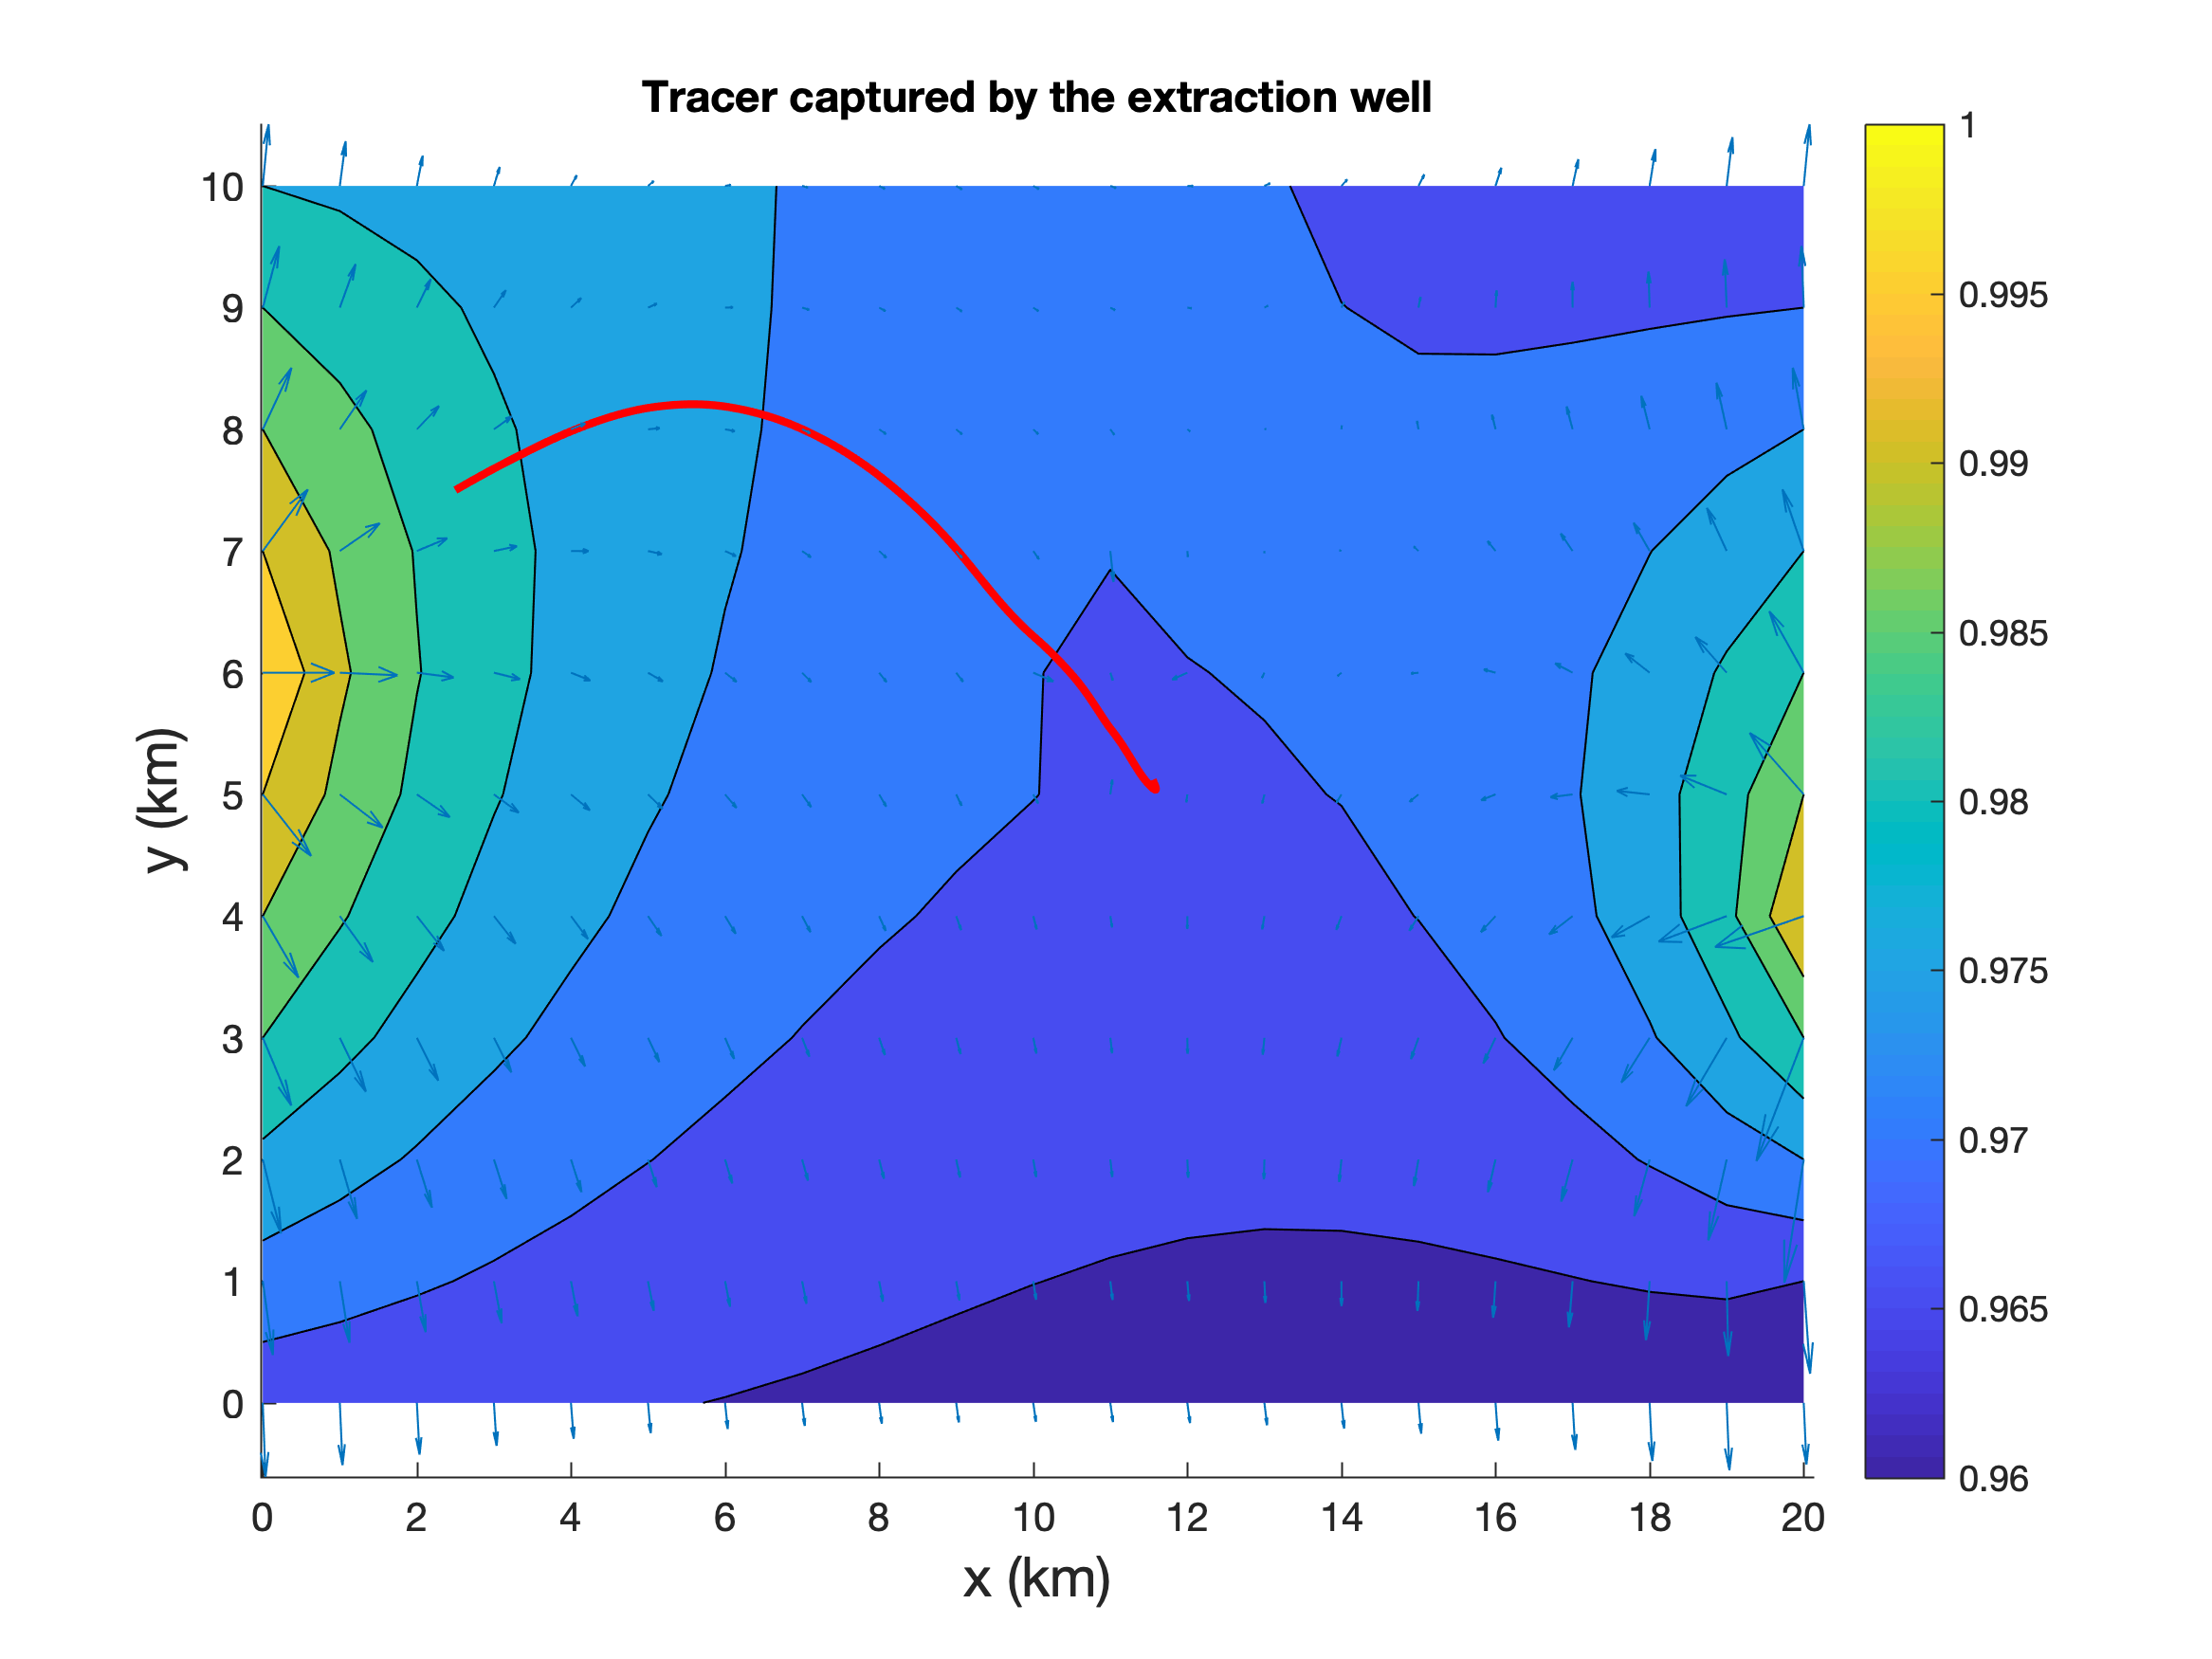
\includegraphics[scale=0.6]{4.png}
    \caption{Tracer captured by the extraction well after 365 days of extraction at the rate of $1.64\times10^{-7} m^2s^{-3}$.}
\end{figure}
\end{document}
